\documentclass{article}\usepackage{graphicx} % new way of doing eps files
\usepackage{listings} % nice code layout
\usepackage[usenames]{color} % color
\usepackage{float}
\definecolor{listinggray}{gray}{0.9}
\definecolor{graphgray}{gray}{0.7}
\definecolor{ans}{rgb}{1,0,0}
\definecolor{blue}{rgb}{0,0,1}
% \Verilog{title}{label}{file}
\newcommand{\Verilog}[3]{
  \lstset{language=Verilog}
  \lstset{backgroundcolor=\color{listinggray},rulecolor=\color{blue}}
  \lstset{linewidth=\textwidth}
  \lstset{commentstyle=\textit, stringstyle=\upshape,showspaces=false}
  \lstset{frame=tb}
  \lstinputlisting[caption={#1},label={#2}]{#3}
}


\author{Christopher Leger}
\title{Lab 2: Adders and Complexity}

\begin{document}
\maketitle

\section{Introduction}
The purpose of this lab was to create multiple methods of addition and subtraction and compare their runtime and complexity. Three different kinds of adders were created and tested and throughout the lab to make their differences apparent. The three kinds are the ripple adder which makes each bit addition after the previous addition, the conditional sum adder which assumes both a zero and a one carry in and then chooses the final result based on the actual carry in, and the last kind is the carry look ahead adder which generates all of the carry first and then calculates all sums simultaneously. 
\section{Interface}
All of the adders take in the same inputs and outputs. Each has two "bits" long inputs, which for this lab "bits" is eight bits to represent the two numbers being added or subtracted. Then each adder has two different one bit inputs which are mode and ci, which are whether it is an adder or subtracter and what the carry in is, respectively. For the outputs, each adder has a "bits" long output called sum which is the sum of the adder and a one bit output called cout which is the overall carry out of the adder.
\section{Design}
The three adders, ripple, conditional sum, and carry look ahead, each have a different design with different benefits and drawbacks for each one. First, the ripple adder uses a series of various types of gates to calculate each sum based on the inputs and the carry from the previous result. The carry propagation causes each sum to need to wait for the previous sum and carry to be calculated and the schematic can be seen in Figure~\ref{fig:rippleadderSch}. Next, the conditional sum adder generates several 2 bit answers using half and full adders, then uses a series of muxs and combining wires to use the first bit of previous answers to choose which answer to use in a different part eventually leading to a correct answer. The schematic can be seen in Figure~\ref{fig:CondSumSch}. Finally, the Carry look ahead uses two blocks of a set number of logic gate levels which will use equations that create generate values, propagate values, and then uses those to calculate values recursively to be used to calculate the carry values which are then used to calculate the final sum values. The carry out of the first block is then used as the carry in of the second block. The schematic for the carry look ahead adder is in Figure~\ref{fig:CarryLookAheadSch}.

\begin{figure}[H]
\begin{center}
	\caption{Design for Ripple adder.}\label{fig:rippleadderSch}
	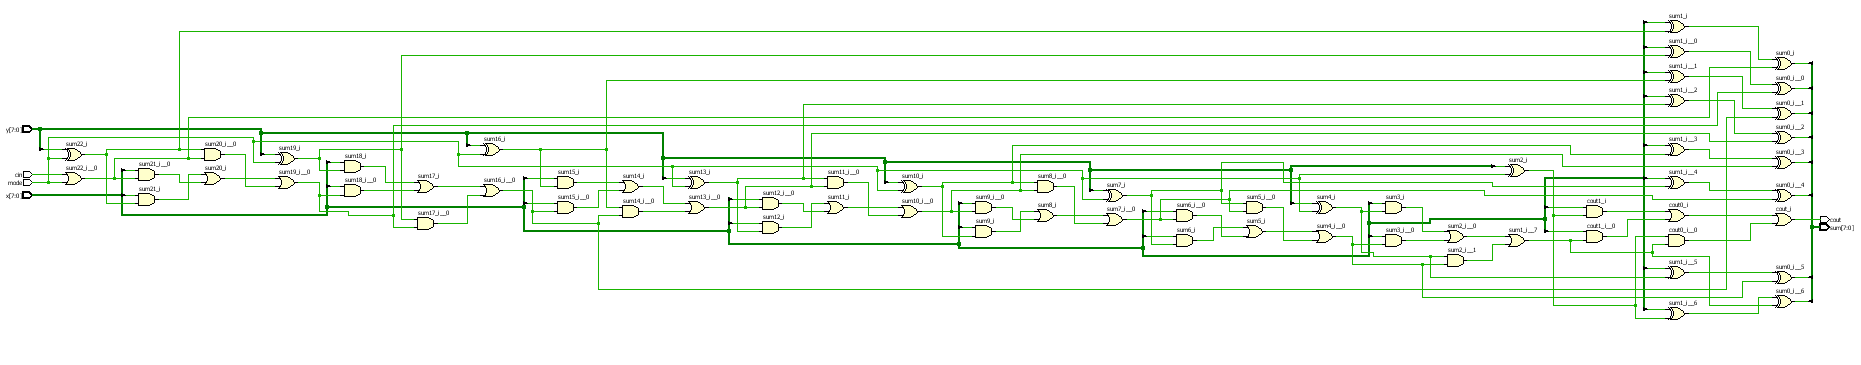
\includegraphics[width=1.2\textwidth]{../images/RippleSch.png}
\end{center}
\end{figure}
\begin{figure}[H]
\begin{center}
	\caption{Design for Conditional Sum adder.}\label{fig:CondSumSch}
	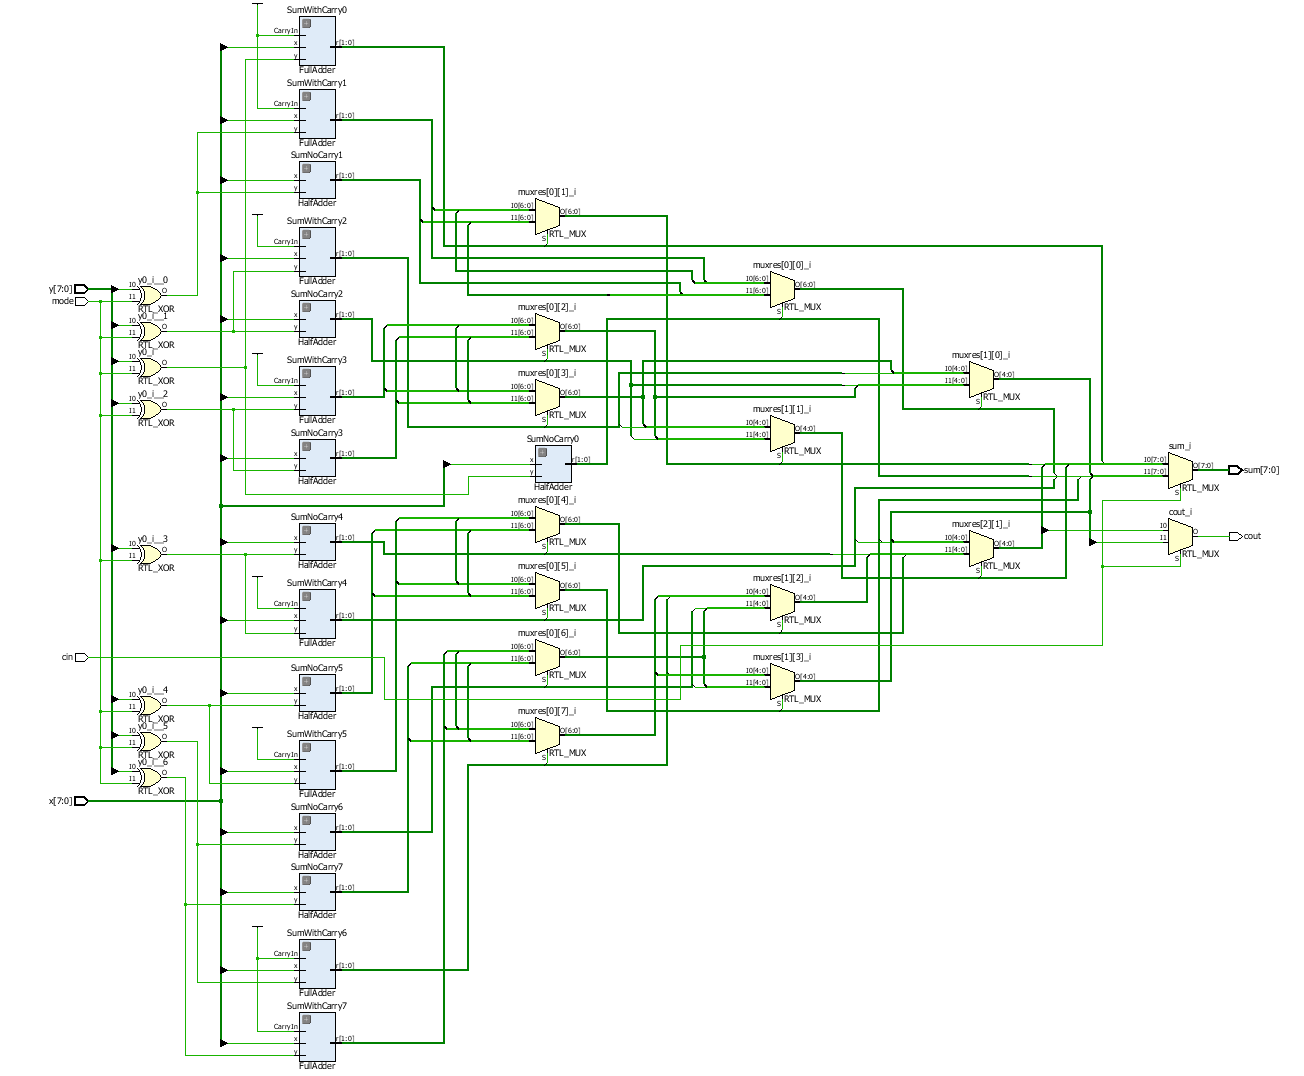
\includegraphics[width=1.2\textwidth]{../images/CSadderSch.png}
\end{center}
\end{figure}
\begin{figure}[H]
\begin{center}
	\caption{Design for Carry Look Ahead adder with 4 bit blocks.}\label{fig:CarryLookAheadSch}
	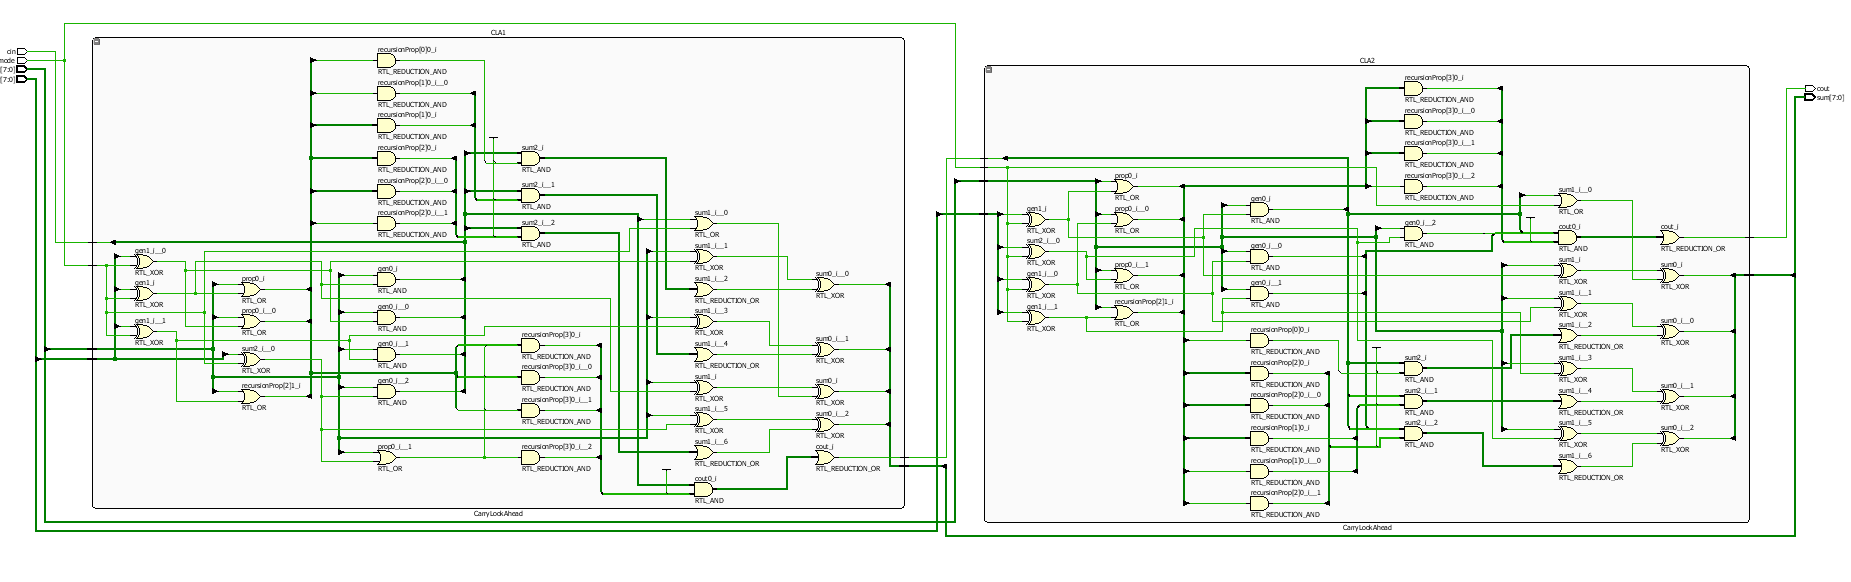
\includegraphics[width=1.2\textwidth]{../images/CarryLookAheadBlocksSch.png}
\end{center}
\end{figure}

\section{Implementation}
Two of the adders are implemented in similar way using a generate statement and for loops to create the propagation of each of the values. The conditional sum adder uses many module calls and assign statements to calculate its answer. The ripple adder first assigns values to the first carry used and the carry out (which is calculated later) then uses a generate statement to create a for loop to flip y based on the mode, calculate the next carry using AND and OR gates using the current bits and the current carry and finally calculates the current sum bit using the current input bits and the current carry. The code for the ripple is seen in Listing~\ref{code:Rippleadder}. The conditional sum adder first creates all of the necessary 2D wire arrays and then uses half and full adders to generate the first level of answers. Next, muxs are used to determine which of those answers to use in the next level. Those answers are then combined with other parts of previous answers to be used in the next level of muxs slowly increasing the number of bits per level but reducing the number of necessary muxs and combining wires. All of these are given value using assign statements for dataflow design because each level just needs to waits for the previous levels answers. The code for the conditional sum can be found in Listing~\ref{code:Condsum}. Finally, the Carry look ahead adder appears similar to the ripple adder up to the point of assigning preliminary carry in and carry out and calculating the sum values. However, the carry look ahead begins to differ by using a nested for loop to calculate all of the carries all at once and then combining that with the inputs to calculate the sums. Then, in another module, two carry look ahead modules are called and connected using the carry out of one to the carry in of the other and splitting the input bits between them. The codes for the carry look ahead and the blocks of carry look aheads can be found in Listings~\ref{code:CLAadder} and~\ref{code:CLAadderBlocks}. 
	
\Verilog{Verilog code for Ripple adder.}{code:Rippleadder}{../code/adder/ripple.v}
\Verilog{Verilog code for Conditional sum adder.}{code:Condsum}{../code/adder/CSadder.v}
\Verilog{Verilog code for Carry look ahead adder.}{code:CLAadder}{../code/adder/CarryLookAhead.v}
\Verilog{Verilog code for Carry look ahead adder with blocks.}{code:CLAadderBlocks}{../code/adder/CarryLookAheadBlocks.v}

\section{Test Bench Design}
Each of the adders were given the same test cases to make sure that each can accomplish the same tasks and more easily see the differences in the timing of each of the adders. First, a simple case is tested to make sure that each of the carries propagate. Then a random case was given to make sure that the adders can change the carry sometimes and other times not based on the inputs. Next, a case is used to make sure that the carry out acts properly and a case is used to check that the subtracter mode functions. Finally, two more cases are used to check the flipping bits and the just adding with no carries. The test bench shown in Listing~\ref{testbench} is the test bench for the ripple adder but other than which module is called, all the tests are the same.

\Verilog{Verilog code for the test benches.}{code:testbench}{../code/adder/ripple_test.v} 
\section{Simulation}
After simulating each of the adders on the test bench, the differences in the designs becomes significantly more apparent. The ripple adder gets each of the results correctly but takes noticeably longer than the other adders. The propagation in the sum result can also be seen in the first result in the ripple simulation in Figure~\ref{fig:RippleSim}. The Conditonal sum adder gets all of the answers immediately in Figure~\ref{fig:CSadderSim} because all of the logic is combinational so each part is assign a value the moment it gets an answer from the previous level. This answer is not always as fast, taking longer based on the number of input bits. Finally, the Carry look ahead adder has two different results included in Figure~\ref{fig:CarryLookAheadSim} which are with and without the blocks. Both have a delay based on the delays used in the generate loops but the blocks is slightly longer due to waiting for the carry out from the first block needing to calculated before the second block can calculate its answer. The Carry look ahead has intermediate values while it calculates but a correct answer is not guaranteed until a constant time after the values are assigned.

\begin{figure}[H]
\begin{center}
    \caption{Simulation of Ripple adder.}\label{fig:RippleSim}
 	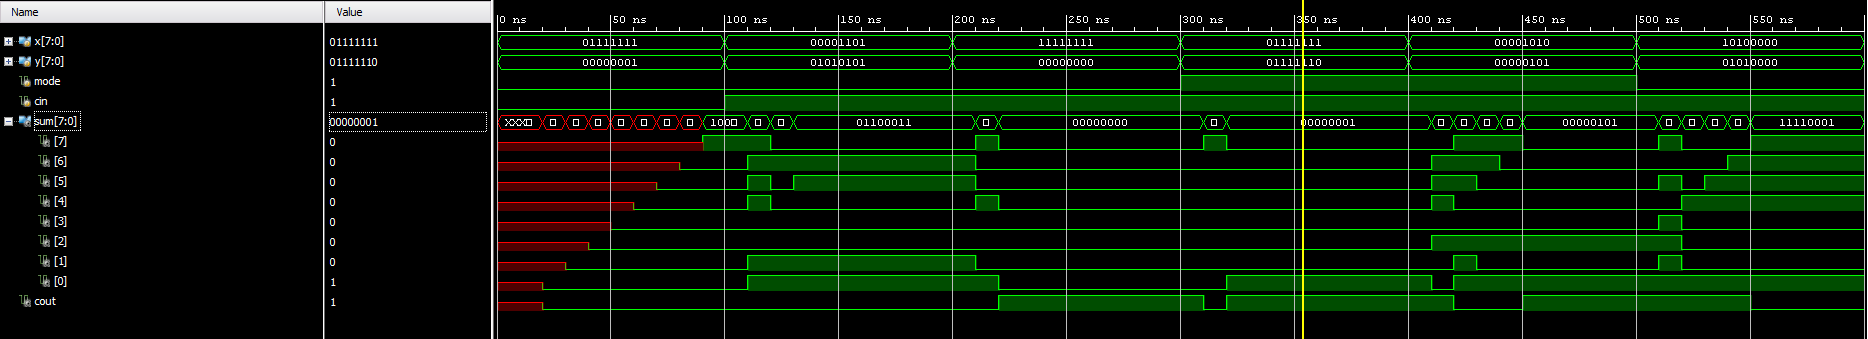
\includegraphics[width=1.2\textwidth]{../images/RippleSim.png}
\end{center}
\end{figure}
\begin{figure}[H]
\begin{center}
 	\caption{Simulation of Condition sum adder.}\label{fig:CSadderSim}
 	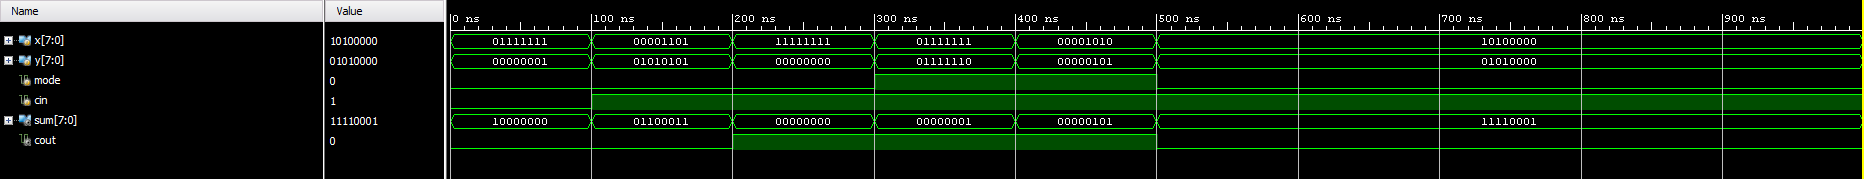
\includegraphics[width=1.2\textwidth]{../images/CSadderSim.png}
\end{center}
\end{figure}
\begin{figure}[H]
\begin{center}
 	\caption{Simulation of Carry look ahead adder.}\label{fig:CarryLookAheadSim}
 	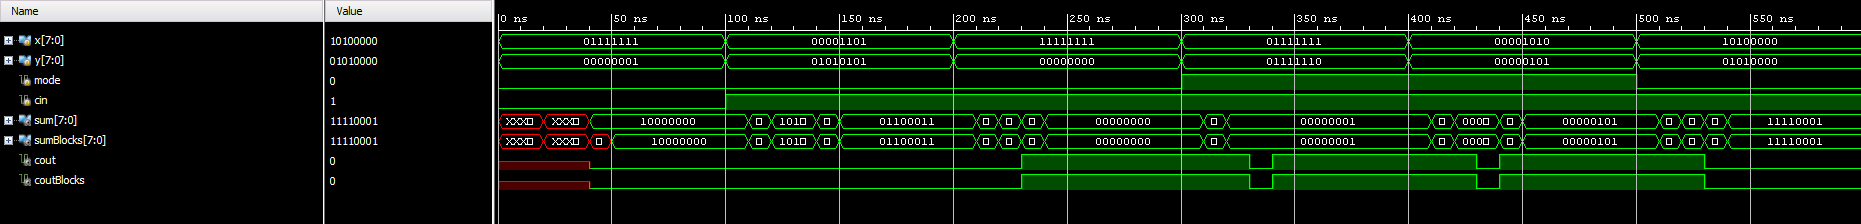
\includegraphics[width=1.2\textwidth]{../images/CarryLookAheadSim.png}
\end{center}
\end{figure}
\section{FPGA Realization and Final Verification}
The FPGA realization was the same for each of the adders as they all have the same inputs and outputs, seen in Listing~\ref{code:FPGA}. The switches were used to provide the inputs with the higher eight being used as x and the lower eight as y. Two buttons were used for the mode and cin with the center button being the mode and the upper button being the cin. Finally, the LEDs were used to provide the output with LEDs 0-7 for the sum and LED 8 for the carry out. All of the adders were verified on the board and each work as expected. With only eight bit inputs it is difficult to see the difference in the time of the output.
\Verilog{Verilog code for FPGA Realization of adders.}{code:FPGA}{../code/adder/AdderPassThrough.v} 
\section{Conclusions}
The objective of this lab was clearly displayed throughout the lab. The ripple adder is the slowest but has the least problem in complexity and fanin. The conditional sum adder is a very complex circuit to implement and has more of a fan in problem than the ripple adder but is significantly faster than ripple. Finally,  the carry look ahead adder has a constant run time meaning that no matter the size of the input, it will give a result in the same about time but, it has a problem with fanin which is usually resolved by breaking the adder into several blocks with smaller inputs.
\end{document} 